\documentclass[12pt,letterpaper]{article}

% =====================
% Configuración general
% =====================
\usepackage[utf8]{inputenc}
\usepackage[T1]{fontenc}
\usepackage[spanish]{babel}
\usepackage{listings}
\usepackage{xcolor}
\usepackage{geometry}
\usepackage{setspace}
\usepackage{titlesec}
\usepackage{fancyhdr}
\usepackage{hyperref}
\usepackage{titlesec}
\usepackage{tabularx}
\usepackage{tocloft}
\usepackage{graphicx}
\usepackage{caption}
\usepackage{tocloft}
\usepackage[backend=biber,style=apa,natbib=true]{biblatex}
% =====================
% --- Bloques de código ---
% =====================
% Definir colores para sintaxis Dart
\definecolor{keywordColor}{RGB}{0,0,180}   % azul para keywords
\definecolor{stringColor}{RGB}{163,21,21}  % rojo para strings
\definecolor{commentColor}{RGB}{0,128,0}   % verde para comentarios

% Configuración de listings para Dart
\lstdefinelanguage{Dart}{
  keywords={abstract, as, assert, async, await, break, case, catch, class, const,
            continue, covariant, default, defer, do, else, enum, export, extends,
            external, factory, false, final, finally, for, Function, get, if, implements,
            import, in, interface, is, late, library, mixin, new, null, on, operator,
            part, required, rethrow, return, set, show, static, super, switch, sync, 
            this, throw, true, try, typedef, var, void, while, with, yield},
  sensitive=true,
  comment=[l]{//},
  morecomment=[s]{/*}{*/},
  string=[b]",
}

\lstset{
  language=Dart,
  basicstyle=\ttfamily\fontsize{11}{13}\selectfont, % Consolas 11pt
  keywordstyle=\color{keywordColor}\bfseries,
  stringstyle=\color{stringColor},
  commentstyle=\color{commentColor}\itshape,
  showstringspaces=false,
  tabsize=4,
  breaklines=true,
  numbers=none,
  frame=single,
  rulecolor=\color{black},
  linewidth=\textwidth,
  framerule=0.1pt,
  xleftmargin=0pt,
  xrightmargin=0pt,
  captionpos=b
}

% =====================
% --- Bibliografía ---
% =====================
\addbibresource{ref.bib}  
\DeclareLanguageMapping{spanish}{spanish-apa}
\hypersetup{
    colorlinks=true,
    linkcolor=black,     % enlaces internos (capítulos, secciones) en negro
    citecolor=black,     % enlaces de citas en negro
    urlcolor=black       % enlaces de URLs en negro
}

% =====================
% --- Márgenes ---
% =====================
\geometry{
  top=2.54cm,
  bottom=2.54cm,
  left=3.17cm,
  right=3.17cm
}

% =====================
% --- Fuente Arial (Helvética) ---
% =====================
\usepackage{helvet}
\renewcommand{\familydefault}{\sfdefault}
\renewcommand\normalsize{\fontsize{11}{13}\selectfont}

% =====================
% --- Espaciado general ---
% =====================
\setstretch{1.5}
\setlength{\parindent}{0pt}
\setlength{\parskip}{16pt}

% =====================
% Encabezado y numeración
% =====================
\pagestyle{fancy}
\fancyhf{} % limpia encabezados/pies
\fancyhead[R]{\thepage} % número de página arriba a la derecha
\renewcommand{\headrulewidth}{0pt} % sin línea inferior

% =====================
% Colores institucionales
% =====================
\definecolor{azulOscuro}{RGB}{54,95,145}  % para Título1
\definecolor{azulClaro}{RGB}{79,129,189}  % para Título2
\definecolor{negro}{RGB}{0,0,0}

% =====================
% --- Formato de Figuras ---
% =====================
\captionsetup[figure]{
    labelfont={bf, color=azulClaro},
    textfont={color=azulClaro, small},
    justification=centering,
    labelsep=space
}

\graphicspath{{img/}}

% =====================
% Formato de Título1 (chapters) y Título2 (sections)
% =====================

% -- Título 1 --
\titleformat{\section}[hang]
  {\bfseries\color{azulOscuro}\fontsize{14}{16}\selectfont}
  {\thesection.}
  {1em}
  {}
\titlespacing*{\section}{0pt}{24pt}{{-16pt}}  % espaciado "antes" 24pt, "después" 12pt

% -- Título 2 --
\titleformat{\subsection}[hang]
  {\bfseries\color{azulClaro}\fontsize{12}{14}\selectfont}
  {\thesubsection.}
  {0.8em}
  {}
\titlespacing*{\subsection}{0pt}{10pt}{{-16pt}}  % espaciado "antes" 10pt, "después" 0pt

% =====================
% Índice de contenidos dinámico
% =====================
\setcounter{tocdepth}{2} % muestra capítulos y secciones en el índice
\hypersetup{
    colorlinks=true,
    linkcolor=negro,
    urlcolor=negro
}

% Hacer que las secciones tengan puntos hasta el número de página
\renewcommand{\cftsecleader}{\cftdotfill{\cftdotsep}}


% =====================
% Índice de figuras dinámico
% =====================
\renewcommand{\cftfigpresnum}{Ilustración\ }
\setlength{\cftfignumwidth}{3cm}
\renewcommand{\cftfigleader}{\cftdotfill{\cftdotsep}}

% =====================
% Documento
% =====================
\begin{document}
\renewcommand{\figurename}{Ilustración} 
{\textbf{\textcolor{azulOscuro}{INFORME TAREA 1}}}

%===========================================================
%===========================================================
% --- Tabla de Datos ---
%===========================================================
%===========================================================

{\setlength{\parskip}{0pt}
\section{Datos Generales}
}

\begin{tabularx}{\textwidth}{|>{\raggedright\arraybackslash}X|>{\raggedright\arraybackslash}X|}
\hline
Título del Informe: & Creación y ejecución de un proyecto \\
\hline
Autor(a): & Carlos Hernández, Olivier Paspuel, Antonio Revilla, Frederick Tipán\\
\hline
Carrera: & Ingeniería en Software \\
\hline
Asignatura o Proyecto: & Desarrollo de Aplicaciones Móviles \\
\hline
Tutor o Supervisor: & Mgtr. Doris Karina Chicaiza Angamarca\\
\hline
Institución: & Universidad de las Fuerzas Armadas ESPE – Matriz Sangolquí \\
\hline
Fecha de entrega: & 23 de octubre de 2025 \\
\hline
\end{tabularx}


%===========================================================
%===========================================================
% --- Introducción ---
%===========================================================
%===========================================================

\section{Introducción}

El siguiente informe presenta el desarrollo de 5 aplicaciones simples en Flutter, el cual es un framework del lenguaje de programación Dart para el desarrollo de aplicaciones móviles multiplataforma. Dichas aplicaciones permitieron distintas maneras de implementar una solución haciendo uso de las herramientas del framework.

Para el desarrollo de cada uno de los ejercicios propuestos, se utilizó el framework Flutter para generar una aplicación móvil multiplataforma visualmente atractiva. Adicionalmente, se utilizaron los IDEs de Visual Studio Code y Andorid Studio para compilar y ejecutar cada aplicación, junto con un emulador de teléfono correspondiente.

Los 5 ejercicios realizados, permitieron familiarizarse con las herramientas que proporciona Flutter para generar interfaces de usuario en dispositivos móviles. También, cada ejercicio permitió elaborar algoritmos que hacen uso eficiente de estructuras como listas, mapas y los distintos tipos de datos que ofrece el lenguaje de programación Dart.

\newpage

%===========================================================
%===========================================================
% --- índice de Contenidos y Figuras ---
%===========================================================
%===========================================================

\renewcommand{\contentsname}{Índice de Contenidos}
{\setlength{\parskip}{0pt}
\tableofcontents
}

\vspace{1.0cm}

\renewcommand{\listfigurename}{Índice de Ilustraciones}
{\setlength{\cftbeforefigskip}{2pt}
\listoffigures
}

\newpage

%===========================================================
%===========================================================
% --- Objetivos ---
%===========================================================
%===========================================================

\section{Objetivos}
\subsection{Objetivo General}
Elaborar un proyecto donde se puedan ejecutar 5 programas distintos en un entorno móvil con Flutter, las cuales permitan explorar las herramientas que ofrece el framework.

\subsection{Objetivo Específicos}
- Reconocer los principales Widgets de Flutter para elaborar interfaces de usuario que tomen, procesen y presenten datos.

- Hacer uso de estados para el manejo dinámico de la presentación de elementos visuales de la interfaz de usuario.

- Utilizar una estructura de carpetas adecuada para organizar código referente a diseño y lógica de programación.

%===========================================================
%===========================================================
% --- Marco Teórico ---
%===========================================================
%===========================================================

\section{Marco Teórico}
\subsection{Widgets en Flutter}
El componente principal de toda aplicación de Flutter, son los Widgets. Estas piezas de código funcionan como bloques de construcción para crear interfaces de usuario (UI). Los widgets se organizan en base a una jerarquía, donde cada widget se anida dentro de otro widget, es de esta manera se genera una especie de “árbol de widgets”, donde cada widget puede obtener un contexto de su padre. \parencite{FlutterDocs2025}

Comúnmente se suele relacionar a los widgets con componentes estructurales definidos, como textos, botones, labels o demás. Lo cierto, es que los widgets son una estructura más compleja, con la cual es capaz de mostrar contenido, establecer temas, ajustar layouts, pero sobre todo, manejar interacciones con el usuario. \parencite{Gill2025}

Al momento de crear un widget, se tiene que generar una clase que herede las características del componente “statelessWidget” o “statefulWidget”. En cualquiera de los casos se \textbf{hereda atributo “key”:} Es un identificador único que ayuda a actualizar secciones específicas de la UI.

\subsection{Stateless widgets}
Es el tipo de widget más simple, pues se lo utiliza cuando el estado del mismo no debe ser mutable, es decir, sus atributos no cambian durante la compilación, por lo que se tendrá el mismo elemento durante toda la aplicación desde que se crea el widget.

Así, este tipo de widget solo implementa el método “build()” que contiene la estructura del widget, por lo que lo convierte en una solución bastante simple, fácil de predecir y optimizada en rendimiento. \parencite{Tllez2024}


\subsection{Stateful widgets}
Este tipo de widget que es capaz de cambiar luego de haber tenido alguna interacción por parte del usuario u otros medios. Para lograr alcanzar esto, se implementa el método “createState()” que sirve para crear un estado del widget declarado. Este estado se lo alacena en una clase separada que hereda la clase “State”. \parencite{Nwogu2023}

Cuando se almacena el estado del widget, se tiene un ciclo de vida, además del “createState()” con el cual se inicializa el widget por primera vez, se compone de los métodos:

\begin{itemize}
  \item \textbf{initState():} Se llama antes de que sea agregado al árbol de widgets, ocurre la inicialización del widget.
  \item \textbf{build():} Contiene la estructura del widget, considerando que será llamado cada vez que se tenga que volver a construir el widget cuando se cambia de estado.
  \item \textbf{setState():} Actualiza el estado del widget, lo que puede involucrar otras variables internas declaradas dentro del estado, es donde se implementa la lógica que posteriormente se verá reflejada en la UI.
  \item \textbf{dispose():} Este método se llama cuando el widget es eliminado del árbol de widgets, elimina cualquiera de los recursos usados por el widget.
\end{itemize}

\subsection{Tipos de widgets}
Existen varios widgets con diferentes propiedades cada uno. Algunos ofrecen mayores capacidades de personalización, por lo que en conjunto pueden lograr armar una UI coherente. \parencite{Pandya2025}

\textbf{Layout:} Define como los widgets se organizan en la pantalla. (\lstinline{Row}, \lstinline{Column}, \lstinline{Stack}, \lstinline{Expanded}, \lstinline{Container})

\textbf{Estructurales:} Proporciona una estructura básica (genérica) para la presentación de la aplicación. (\lstinline{Scaffold}, \lstinline{AppBar}, \lstinline{Drawer})


\textbf{Interactivos:} Permiten a las personas interactuar con la aplicación. (\lstinline{ElevatedButton}, \lstinline{TextButton}, \lstinline{IconButton}, \lstinline{TextField}, \lstinline{Checkbox}, \lstinline{Switch}, \lstinline{Radio})


\textbf{Widgets espeíficos de plataforma:} Se encuentran los ``Material widgets'' para Android y los ``Cupertino widgets'' para iOS, con la finalidad de tener experiencias más parecidas a como si hubiesen sido hechas nativamente.


\textbf{Estilos:} Ayudan a controlar la apariencia del diseño. (\lstinline{Padding}, \lstinline{Align}, \lstinline{Them}, \lstinline{DecoratedBox})



%===========================================================
%===========================================================
% --- Desarollo ---
%===========================================================
%===========================================================

\section{Desarrollo}

El proyecto se encuentra cargado en el siguiente repositorio de GitHub: 

\href{https://github.com/vieerr/multipurpose-app}{\color{blue}\underline{https://github.com/vieerr/multipurpose-app}}

\subsection{Esctructura del proyecto}
El proyecto se desarrolló bajo el nombre \lstinline{multipurpose-app}, y desde el principio se organizaron las carpetas de manera que cada sección del proyecto quedara clara y ordenada. Esto no solo ayuda a mantener todo estructurado, sino que también hace que implementar los distintos módulos sea mucho más sencillo y ágil.

\begin{figure}[H]
    \centering
    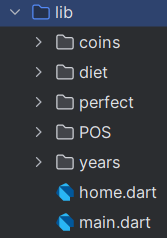
\includegraphics[width=0.4 \textwidth, height=5cm, keepaspectratio]{estructura_proy.png}
    \caption{Estructura de carpetas de proyecto}
    \label{fig:strpry}
\end{figure}

La navegación dentro de la app se maneja desde \lstinline{home.dart} usando una barra inferior, el \lstinline{NavigationBar}, que facilita moverse entre los distintos módulos. Para saber qué pantalla está activa en cada momento, se usa la variable \lstinline{currentPageIndex}. Cada vez que el usuario toca una de las pestañas, el método \lstinline{onDestinationSelected} actualiza ese índice, y gracias a eso el body del \lstinline{Scaffold} se encarga de mostrar dinámicamente el widget que corresponde a la sección seleccionada.

La interfaz también cuenta con una barra superior, o \lstinline{AppBar}, donde se muestra el título de la aplicación junto con algunos accesos rápidos. Al trabajar con un \lstinline{StatefulWidget}, cada módulo puede conservar su propio estado de manera independiente, lo que significa que las transiciones entre secciones son suaves y cada parte de la app funciona de forma autónoma sin interferir con las demás.


\subsection{Ejercicio 11 (POS)}
Implementación de código 11



\subsection{Ejercicio 12 (coins)}
Texto desde un lado



\subsection{Ejercicio 1 (years)}
Contenido desde un archivo a parte

\subsection{Ejercicio 14 (perfect)}
\textbf{Paso 1: Estructuración según el patrón MVC}  
Para estructurar el módulo de números perfectos, se siguió nuevamente el patrón Modelo-Vista-Controlador (MVC). Se crearon archivos separados para el modelo (PerfectNumber), el controlador (PerfectController) y la vista (PerfectPage), lo que mantiene la lógica de cálculo, la gestión de datos y la interfaz de usuario bien diferenciadas y fáciles de mantener dentro del proyecto.
Se crearon tres carpetas principales dentro del proyecto:  
\begin{itemize}
    \item model
    \item view
    \item controller
\end{itemize}

\textbf{Paso 2: Creación de archivos .dart para cada componente}  
Dentro de cada carpeta se añadieron los archivos correspondientes en el siguiente orden de desarrollo:  

\begin{itemize}
    \item \textbf{Model:} 
        \begin{itemize}
            \item perfectModel.dart
        \end{itemize}
    \item \textbf{Controller:} 
        \begin{itemize}
            \item perfectController.dart
        \end{itemize}
    \item \textbf{View:} 
        \begin{itemize}
            \item perfectView.dart
        \end{itemize}
\end{itemize}

\textbf{Paso 3: Desarrollo de los componentes (modelo $\rightarrow$ controlador $\rightarrow$ vista)}  

\textbf{Modelos:}  

\begin{itemize}
    \item \textbf{perfectModel.dart}: La clase \texttt{PerfectNumber} básicamente se dedica a revisar si un número es perfecto, que se base en la programación donde si sumas todos sus divisores (excluyendo el propio número) el resultado es exactamente el mismo número. Al crear una instancia con un número, la clase automáticamente calcula sus divisores y determina si cumple o no con esta condición.

    Dentro de la clase, la lógica se apoya principalmente en dos métodos: \texttt{\_calculateDivisors}, que identifica y ordena todos los divisores menores que el número, y \texttt{\_checkIfPerfect}, que suma esos divisores para confirmar si el número es perfecto. Además, incluye métodos adicionales que hacen posible alcanzar la suma de los divisores y presentarlos como texto, lo que sirve mucho tanto para mostrarlos al usuario como para aprovechar los datos en otras partes de la app.
\end{itemize}

\textbf{Controladores:}  

\begin{itemize}
    \item \textbf{perfectController.dart}: La clase \texttt{PerfectController} gestiona toda la lógica detrás de la verificación de números perfectos. Para ello, importa la clase \texttt{PerfectNumber} y proporciona el método \texttt{checkNumber}, que trabaja con un número, si es mayor que cero, crea una instancia de \texttt{PerfectNumber} para comprobar sus divisores y comprobar si verdaderamente es un número perfecto. De esta manera, el controlador unifica tanto la validación como la creación del modelo, evitando el manejo de información errónea y manteniendo la comunicación clara y ordenada entre la lógica del programa y la interfaz de usuario.
\end{itemize}

\textbf{Vista:}  

\begin{itemize}
    \item \textbf{perfectView.dart}: En este archivo se define la interfaz en Flutter que permite comprobar si un número es perfecto. Para hacerlo, se utiliza un \texttt{NumberField}, donde el usuario ingresa el número, un \texttt{PrimaryButton} que ejecuta la verificación y el componente \texttt{PerfectCard}, que actúa como el enlace entre lo que el usuario introduce y la lógica del \texttt{PerfectController}, encargado de calcular los divisores y determinar si el número cumple la condición.
    
    La página principal, \texttt{PerfectPage}, está construida sobre un \texttt{Scaffold} que integra esta tarjeta de verificación. Lo interesante es que los resultados se actualizan al instante: muestra si el número es perfecto y también la suma de sus divisores. En esencia, esta pantalla conecta de forma directa la interfaz con la lógica del controlador, logrando que la interacción sea fluida y los cálculos se reflejen en tiempo real.
\end{itemize}

\textbf{Paso 4: Integración en la aplicación}  
Para integrar la funcionalidad de números perfectos, lo que hicimos fue importar \texttt{PerfectPage} en el \texttt{Home.dart} y agregarla como una opción más en la lista de secciones.

Así, cuando el usuario elige esta opción en la barra de navegación, la página carga automáticamente y le permite ingresar un número para verificar si es perfecto, mostrando también sus divisores. De esta forma, queda totalmente integrado en la navegación principal de la aplicación.

\subsection{Ejercicio 15 (diet)}

El sistema plantea una estructura de MVC(Modelo-Vista-Controlador). Para poder comprender esto de mejor manera analizaremos cada uno de sus componentes por separado.

\textbf{Modelo}

\begin{itemize}
    \item \textbf{WeightMeasurementModel}
\end{itemize}

\begin{center}
\begin{lstlisting}
class WeightMeasurementModel {
  int id;
  DateTime date;
  List<double> weights;
  double averageWeight;
  double? difference;
  String? state;
}
\end{lstlisting}
\end{center}

Es la instancia de cada medición de peso, en esta almacenamos los 10 valores de las balanzas, su promedio, la diferencia con el último peso registrado o si es la primera medición con el peso inicial ingresado por el usuario. Por último asignamos un valor al estado para saber si en esa medición subió o bajó de peso.

\begin{itemize}
    \item \textbf{PersonModel}
\end{itemize}

\begin{center}
\begin{lstlisting}
class WeightMeasurementModel {
  int id;
  String name;
  double initialWeight;
  List<WeightMeasurementModel> measurements;
}
\end{lstlisting}
\end{center}

Es la instancia de cada persona que va a pesarse, a esta se le asigna un identificador único, un nombre y una lista de mediciones, de esta manera asociamos las mediciones a cada persona y podremos acceder a ellos para usarlos en la vista.

Adicional se calcula el promedio. métodos de ingreso de personas dependiendo si es su primera medición y sirve para poder extraer los datos y mostrarlos en la ui.

\textbf{Controlador}

\begin{center}
\begin{lstlisting}
class PersonController with ChangeNotifier{
  List<PersonModel> _persons = [];
  int _nextPersonId = 1;
\end{lstlisting}
\end{center}

Es el controlador central, este usa change Notifier para poder recargar la ui (especialmente las listas) después de realizar un ingreso de una nueva persona o medida, este controlador maneja la lista central de personas que es la que manejara las nuevas instancias. En esta clase también tenemos las funciones que controlan inserciones y formatos de visualización.

El controlador actúa como una capa intermedia entre los modelos y la interfaz de usuario, permitiendo que los organismos y páginas se mantengan enfocados únicamente en la presentación, sin preocuparse por la gestión del estado o la persistencia temporal de los datos.

\textbf{Flujo General}

El flujo principal inicia en la página DietPage, que representa la pantalla de inicio del sistema. En ella, el usuario encuentra un formulario para registrar una nueva persona y una lista con las personas ya registradas.

El registro de una persona se realiza a través del PersonFormOrganism, donde el usuario ingresa el nombre y el peso inicial. Tras validar el formulario, se invoca al método addPerson del controlador, que crea y almacena una nueva instancia de PersonModel. Luego, el formulario se limpia y la interfaz se actualiza para reflejar el nuevo registro.

La lista de personas registradas se muestra mediante el PersonListOrganism, donde cada persona aparece dentro de una tarjeta (Card) que incluye su nombre y un distintivo de estado (badge) que indica si su peso ha aumentado o disminuido. Al seleccionar una persona, se navega a la vista de detalle (PersonDetailOrganism), donde se pueden consultar las mediciones históricas y registrar nuevas entradas.


%===========================================================
%===========================================================
% --- Conclusiones y Recomendaciones ---
%===========================================================
%===========================================================

\section{Conclusiones y Recomendaciones}
\subsection{Conclusiones}

\begin{itemize}
    \item Se logró desarrollar una aplicación móvil con el framework de Flutter en la cual se agrega un sistema de navegación para moverse entre cinco ejercicios diferentes. Esto permitió cumplir con el objetivo de explorar a fondo las herramientas que ofrece el framework y poner en práctica, los conceptos relacionados con el diseño y desarrollo de interfaces para dispositivos móviles.
    \item Se reconocieron y utilizaron en el desarrollo de la aplicación los Widgets más relevantes de Flutter. Esto permitió crear interfaces interactivas que presentan y capturan datos de forma clara y eficiente.
    \item Se trabajó con el manejo de estados dentro de las aplicaciones para que los elementos de la interfaz pudieran actualizarse de manera dinámica, respondiendo a los cambios en tiempo real. Gracias a esto, se logró controlar la presentación de la información de forma ágil y adaptable.
    \item Se organizó el código de forma clara, separando en carpetas distintas lo que corresponde al diseño y lo que corresponde a la lógica de programación. De esta manera, se siguieron buenas prácticas en la fase de desarrollo y también se siguieron buenas practicas de organización.
    \item Aplicar los principios de Atomic Design, permitio crear interfaces de manera modular, lo que las hizo más fáciles de reutilizar y escalar. Esto permitió organizar claramente los componentes en diferentes niveles como: átomos, moléculas y organismos, lo que simplifica y mejora el desarrollo ademas de mejorar el mantenimiento de la aplicación.
    \item Al aplicar el patrón MVC (Modelo-Vista-Controlador), se logró mantener la lógica de negocio separada de la parte visual de la aplicación, lo que hizo que el código fuera más claro y también hace que el codigo sea mas mantenible y organizado.
\end{itemize}


\subsection{Recomendaciones}

\begin{itemize}
    \item Se recomienda continuar aplicando en futuros proyectos la metodología de Atomic Design, porque ayuda a crear interfaces que son modulares, escalables y fáciles de reutilizar. Mantener este enfoque hace que agregar nuevos componentes o ampliar la aplicación sea mucho más sencillo, sin alterar la estructura de lo que ya está funcionando.
    
    \item Es importante seguir utilizando el patrón MVC (Modelo-Vista-Controlador) en proyectos donde se pueda aplicar, ya que las diferentes caracteristicas y beneficios que brinda como: separar la lógica de negocio de la presentación. No solo hace que el código sea más claro y fácil de mantener, sino que también simplifica la incorporación de nuevas funciones, ademas este patrón puede facilitar proyectos más complejos.
    
    \item Se recomienda documentar y estandarizar los componentes y Widgets creados en las aplicaciones, enfocándose en que puedan reutilizarse dentro del mismo proyecto o incluso en otros proyectos. Esto permite aprovechar al máximo la modularidad que ofrece Atomic Design y la clara separación de responsabilidades que da el patrón MVC, garantizando consistencia, un mantenimiento más sencillo y la posibilidad de escalar la aplicación sin tener muchos problemas.
\end{itemize}


%===========================================================
%===========================================================
% --- Referencias Bibliográficas ---
%===========================================================
%===========================================================

\section{Referencias Bibliográficas}
\printbibliography[heading=none]

%===========================================================
%===========================================================
% --- Anexos ---
%===========================================================
%===========================================================

\section{Anexos}
Anexo 1 Pasos del instalador de Android estudio


\end{document}
